% example tikz figure

\documentclass{standalone}
\usepackage{amsmath}
\usepackage{tikz}
\usetikzlibrary{arrows,shapes,positioning,shadows,trees}


\begin{document}
\tikz \node [scale=0.8, inner sep=0] {
\begin{tikzpicture}
    \node (a) at (0,0) {
        \begin{tikzpicture}
            % fill rectangle
            \filldraw[fill=gray!20,draw=white] (-2,1) rectangle (2,-1);
            % draw axis with no labels, size 4x4
            \draw[-] (-2,0) -- (2,0);
            \draw[-] (0,-2) -- (0,2);
            \draw[-] (-2,1) -- (2,1);
            \draw[-] (-2,-1) -- (2,-1);

            % label the corners of the square, using the anchor points
            \node[anchor=south west] at (0,1) {$i\theta$};
        \end{tikzpicture}
    };

    \node (b) at (8,0) {
        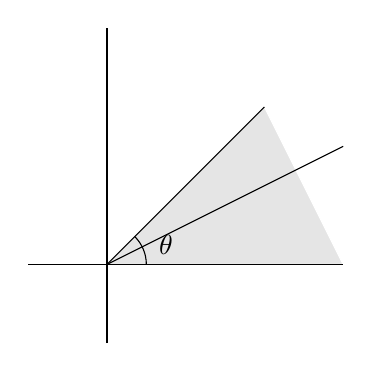
\begin{tikzpicture}
            % fill triangle
            \filldraw[fill=gray!20,draw=white] (0,0) -- (2,2) -- (3,0) -- (0,0);
            \draw[-] (-1,0) -- (3,0);
            \draw[-] (0,-1) -- (0,3);
            \draw[-] (0,0) -- (2,2);
            \draw[-] (0,0) -- (3,1.5);
            % label pi/4 as arc at center
            \draw (0.5,0) arc (0:45:0.5);
            \node at (0.75,0.25) {$\theta$};
        \end{tikzpicture}
    };

    % label two arrows:
    % from a to b, label on top as e^{z}
    % from b to a, label on bottom as log z

    \draw[->] (a) -- (b) node[midway,above] {$e^z$};
    \draw[->] (b) -- (a) node[midway,below] {$\log z$};

    \node (c) at (16,0) {
        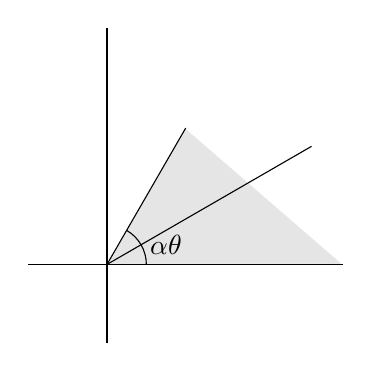
\begin{tikzpicture}
            % copy from node b, but make the angle from pi/4 to pi/3

            % fill triangle
            \filldraw[fill=gray!20,draw=white] (0,0) -- (1,1.732) -- (3,0) -- (0,0);
            \draw[-] (-1,0) -- (3,0);
            \draw[-] (0,-1) -- (0,3);
            \draw[-] (0,0) -- (1,1.732);
            \draw[-] (0,0) -- (1.732 * 1.5,1 * 1.5);
            % label pi/3 as arc at center
            \draw (0.5,0) arc (0:60:0.5);
            \node at (0.75,0.25) {$\alpha\theta$};
        \end{tikzpicture}
    };

    % label from b to c
    \draw[->] (b) -- (c) node[midway,above] {$z^{\alpha} (\alpha > 0)$};
\end{tikzpicture}
};

\tikz \node [scale=0.8, inner sep=0] {
    \begin{tikzpicture}
        \node (a) at (0,0) {
            \begin{tikzpicture}
                % fill -i, B, i, A with arc
                \filldraw[fill=gray!20,draw=white] (0,-1) -- (1.732, 0) arc (30:150:2) -- (0,-1);
                % draw axis with no labels, size 4x4
                \draw[->] (-3,0) -- (3,0);
                \draw[->] (0,-3.5) -- (0,3);

                % draw circle from (0,-1) radius 2
                \draw (0,-1) circle (2);

                % label -i
                \node[anchor=north west] at (0,-1) {$-i$};
                % label i
                \node[anchor=south west] at (0,1) {$i$};
                % label B at sqrt 3
                \node[anchor=south west] at (1.732,0) {$B$};
                % label A at -sqrt 3
                \node[anchor=south east] at (-1.732,0) {$A$};
                % tangent line at A
                \draw[dashed] (-1.732 - 1, -1.732) -- (-1.732 + 1, 1.732);
            \end{tikzpicture}
        };


        \node (b) at (8,0) {
            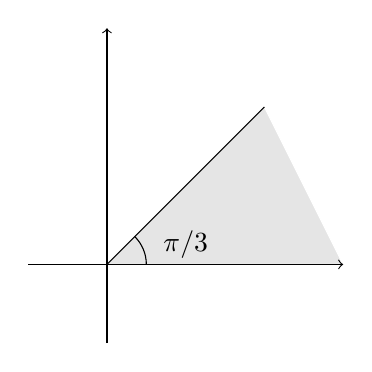
\begin{tikzpicture}
                % fill triangle
                \filldraw[fill=gray!20,draw=white] (0,0) -- (2,2) -- (3,0) -- (0,0);
                \draw[->] (-1,0) -- (3,0);
                \draw[->] (0,-1) -- (0,3);
                \draw[-] (0,0) -- (2,2);
                % label pi/4 as arc at center
                \draw (0.5,0) arc (0:45:0.5);
                \node at (1,0.25) {$\pi / 3$};
            \end{tikzpicture}
        };

        \node (c) at (16,0) {
            
\begin{tikzpicture}
                \filldraw[fill=gray!20,draw=white] (-2,0) -- (2,0) -- (2,1) -- (-2,1) -- (-2,0);
                \draw[-] (-2,0) -- (2,0);
            \end{tikzpicture}
        };

        \node (d) at (24,0) {
            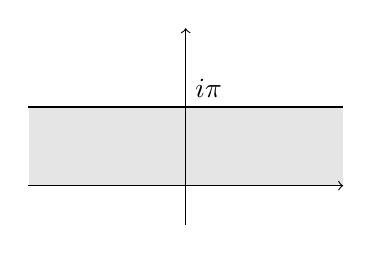
\begin{tikzpicture}
                % fill rectangle
                \filldraw[fill=gray!20,draw=white] (-2,1) rectangle (2,0);
                % draw axis with no labels, size 4x4
                \draw[->] (-2,0) -- (2,0);
                \draw[->] (0,-0.5) -- (0,2);
                \draw[-] (-2,1) -- (2,1);

                % label the corners of the square, using the anchor points
                \node[anchor=south west] at (0,1) {$i\pi$};
            \end{tikzpicture}
        };

        \draw[->] (a) -- (b) node[midway,above] {$g(z) = - \dfrac{z+\sqrt{3}}{z-\sqrt{3}}$};
        \draw[->] (a) -- (b) node[midway,below] {$g(i) = - \dfrac{i+\sqrt{3}}{i-\sqrt{3}}$};
        \draw[->] (b) -- (c) node[midway,above] {$z^3$};
        \draw[->] (c) -- (d) node[midway,above] {$\log z$};
    \end{tikzpicture}
};
\end{document}